% Provenance (never printed): see sources/outline_sources.md (Year 1:
% geological cross-sections, apparent dip, thickness, boreholes). Every
% Varden Hills number comes from figdata/bachelor-1/varden_sections.py, which
% imports the shared model figdata/shared/region.py; numbers of the exercises
% and problem in the Book 3 scratch calculator and in that script's values.
\chapter{Les coupes géologiques}\label{ch:b1:cross-sections}

Une société d'ingénierie prévoit un tunnel sous les collines de Varden, droit de
l'ouest vers l'est à une altitude constante de \qty{200}{m}. Avant qu'un seul
mètre soit creusé, les géologues doivent dire quelles roches la machine va
couper, où elle traversera la faille, et combien de temps elle passera dans le
calcaire, roche susceptible de contenir des cavités ouvertes et de l'eau.
Personne ne peut voir l'intérieur des collines~; mais la \omterm{def:b1:geological-maps:geological-map}{carte géologique} du
\cref{ch:b1:geological-maps}, quelques sondages et la géométrie des plans
suffisent à dessiner une tranche verticale du sous-sol --- une \omterm{def:b1:cross-sections:section}{coupe
géologique} --- et à y lire les réponses. Ce chapitre enseigne comment on
construit une coupe à partir d'une carte, comment les \omterm{def:b1:geological-maps:attitude}{pendages} et les épaisseurs
changent quand la tranche est coupée en oblique, comment on corrèle les
sondages, et comment une coupe raconte l'histoire des roches qu'elle recoupe. Il
se termine par le tunnel.

\begin{recall}
L'\omterm{def:b1:geological-maps:attitude}{attitude} d'un plan est donnée par son \omterm{def:b1:geological-maps:attitude}{sens du pendage} $\alpha$ et son \omterm{def:b1:geological-maps:attitude}{pendage}
$\delta$, et le plan passant par un point d'altitude $z_0$ situé à l'origine est
$z = z_0 - \tan\delta\,(x\sin\alpha + y\cos\alpha)$~; trois points d'un contact
fixent son \omterm{def:b1:geological-maps:attitude}{attitude}~; la règle des V lit le \omterm{def:b1:geological-maps:attitude}{pendage} sur la figure d'\omterm{def:b1:geological-maps:geological-map}{affleurement}
dans les vallées (\cref{ch:b1:geological-maps}). Une courbe de niveau joint les
points de même altitude sur une carte topographique (livre~1, année~9). Les
roches plus jeunes reposent sur les plus anciennes, et ce qui recoupe une roche
est plus jeune qu'elle (livre~1, année~7).
\end{recall}

\section{De la carte à la coupe}

\begin{definition}[Coupe géologique, profil topographique, exagération verticale]\label{def:b1:cross-sections:section}
Une \emph{coupe géologique}\index{coupe geologique@coupe géologique} est un dessin des unités rocheuses et des structures
dans un plan vertical du sous-sol, le long d'une ligne tracée sur la carte. Son
bord supérieur est le \emph{profil topographique}\index{profil topographique},
la courbe de l'altitude du sol le long de la ligne. L'\emph{exagération
verticale}\index{exageration verticale@exagération verticale} $e$ d'une coupe est le rapport de son échelle verticale à son
échelle horizontale~; une coupe est \emph{à l'échelle vraie} lorsque $e = 1$.
\end{definition}

\begin{method}[Construire une coupe à partir d'une carte]\label{met:b1:cross-sections:construct}
\begin{enumerate}
  \item Tracer la ligne de coupe sur la carte et poser le bord d'une bande de
        papier le long de celle-ci~; marquer l'endroit où chaque courbe de niveau
        la coupe, avec son altitude, et l'endroit où chaque contact et chaque
        faille la coupe.
  \item Tracer une ligne de base horizontale de même longueur et une échelle
        verticale d'altitude (choisir $e$, et l'inscrire sur la coupe).
  \item Reporter chaque repère de courbe de niveau à son altitude et joindre les
        points en courbe régulière~: c'est le \omterm{def:b1:cross-sections:section}{profil topographique}.
  \item Reporter chaque contact et chaque faille sur le profil, au point où elle
        coupe la ligne.
  \item De chacun de ces points, prolonger le contact dans le sol avec son
        \omterm{def:b1:geological-maps:attitude}{pendage} \emph{dans le plan de la coupe} --- son \omterm{def:b1:cross-sections:apparent-dip}{pendage apparent}
        (\cref{sec:b1:cross-sections:apparent}) --- exagéré du facteur $e$ si
        $e \ne 1$~; utiliser les sondages et les \omterm{def:b1:cross-sections:structure-contour}{isohypses structurales} là où il
        y en a.
  \item Compléter les unités entre les \omterm{def:b1:geological-maps:geological-map}{contacts}, en respectant l'ordre de
        superposition et les recoupements, et ajouter la légende, les échelles,
        l'orientation de la ligne et $e$.
\end{enumerate}
\end{method}

\begin{omfigure}
\begin{tikzpicture}[font=\scriptsize, x=1cm, y=1cm]
% map strip with contours crossing the section line
\draw[black!50] (0,2.7) rectangle (9,4.5);
\foreach \x/\h in {0.7/300, 1.6/350, 2.6/400, 4.1/400, 5.0/350, 5.8/300, 7.2/300, 8.2/350} {
  \draw[contour, brown!70!black] (\x-0.25,2.7) .. controls (\x+0.1,3.4) and (\x-0.1,3.8) .. (\x+0.2,4.5);
  \node[brown!60!black, above] at (\x+0.2,4.5) {\h};
}
\draw[omThm, thick] (0,3.6) node[left] {X} -- (9,3.6) node[right] {Y};
\fill[omDef] (3.4,3.6) circle (1.5pt);
\node[omDef, fill=white, inner sep=1pt, above right] at (3.4,3.62) {contact};
% profile
\draw[->] (0,-0.1) -- (0,1.95) node[above] {altitude (m)};
\draw (0,0) -- (9,0);
\foreach \y/\l in {0/250, 0.5/300, 1.0/350, 1.5/400} { \draw (-0.08,\y) -- (0,\y); \node[left] at (-0.08,\y) {\l}; }
\coordinate (p1) at (0.85,0.5); \coordinate (p2) at (1.75,1.0); \coordinate (p3) at (2.75,1.5);
\coordinate (p4) at (4.25,1.5); \coordinate (p5) at (5.15,1.0); \coordinate (p6) at (5.95,0.5);
\coordinate (p7) at (7.35,0.5); \coordinate (p8) at (8.35,1.0);
\foreach \i/\x in {1/0.85,2/1.75,3/2.75,4/4.25,5/5.15,6/5.95,7/7.35,8/8.35} {
  \draw[black!35, densely dotted] (\x,3.6) -- (p\i);
  \fill (p\i) circle (1.2pt);
}
\draw[thick] (0,0.2) .. controls (0.5,0.3) .. (p1) .. controls (1.3,0.8) .. (p2) .. controls (2.3,1.35) .. (p3)
  .. controls (3.5,1.85) .. (p4) .. controls (4.7,1.25) .. (p5) .. controls (5.5,0.7) .. (p6)
  .. controls (6.6,0.25) .. (p7) .. controls (7.9,0.75) .. (p8) .. controls (8.7,1.15) .. (9,1.2);
\draw[omDef, densely dotted] (3.4,3.6) -- (3.4,1.72);
\draw[omDef, thick] (3.4,1.72) -- (4.45,0.05);
\node[omDef, below right] at (4.3,-0.02) {contact, tracé avec son pendage apparent};
\end{tikzpicture}

{\small Construction d'une coupe (schématique)~: les points où les courbes de
niveau coupent la ligne X--Y sont reportés à leurs altitudes pour donner le
\omterm{def:b1:cross-sections:section}{profil topographique}~; un contact qui coupe la ligne est reporté sur le profil et
prolongé dans le sol avec son \omterm{def:b1:cross-sections:apparent-dip}{pendage apparent}.}
\end{omfigure}

La coupe ci-dessous a été construite par ordinateur à partir du modèle des
collines de Varden le long de la ligne C--D, qui traverse la carte plein est à
$y = \qty{6}{km}$. Elle montre l'\omterm{def:b1:geological-maps:fold}{anticlinal} dont le cœur de grès et de socle
apparaît vers $x \approx \qty{3.5}{km}$, le calcaire et l'argilite sur ses
flancs, la craie dans le \omterm{def:b1:geological-maps:fold}{synclinal} à l'est, et la faille normale. La ligne du
tunnel, à \qty{200}{m}, et les sondages B1, B2, B3 de la
\cref{sec:b1:cross-sections:boreholes} y sont dessinés.

\begin{omfigure}
\begin{tikzpicture}
\begin{axis}[x=1.4cm, y=0.0042cm, xmin=0, xmax=10, ymin=-500, ymax=650,
  axis on top, tick label style={font=\scriptsize}, label style={font=\small},
  xlabel={distance vers l'est depuis C (km)}, ylabel={altitude (m)},
  ytick={-400,-200,0,200,400,600}, clip=true]
\addplot[lith schist, draw=black, line width=0.3pt, even odd rule] table {figdata/out/bachelor-1-varden_sections-cd-unit-schist.dat};
\addplot[lith granite, draw=black, line width=0.3pt, even odd rule] table {figdata/out/bachelor-1-varden_sections-cd-unit-granite.dat};
\addplot[om lith={icsTriassic!35}{om sand}, draw=black, line width=0.3pt, even odd rule] table {figdata/out/bachelor-1-varden_sections-cd-unit-sandstone.dat};
\addplot[om lith={icsJurassic!40}{om limestone}, draw=black, line width=0.3pt, even odd rule] table {figdata/out/bachelor-1-varden_sections-cd-unit-limestone.dat};
\addplot[om lith={icsJurassic!15}{om shale}, draw=black, line width=0.3pt, even odd rule] table {figdata/out/bachelor-1-varden_sections-cd-unit-shale.dat};
\addplot[om lith={icsCretaceous!35}{om limestone}, draw=black, line width=0.3pt, even odd rule] table {figdata/out/bachelor-1-varden_sections-cd-unit-chalk.dat};
\addplot[lith alluvium, draw=black, line width=0.3pt, even odd rule] table {figdata/out/bachelor-1-varden_sections-cd-unit-alluvium.dat};
\addplot[black, line width=0.8pt] table {figdata/out/bachelor-1-varden_sections-cd-ground.dat};
\addplot[fault, line width=1.1pt] table {figdata/out/bachelor-1-varden_sections-cd-fault.dat};
\addplot[omThm, line width=1.4pt] coordinates {(1,200) (9,200)};
\node[omThm, font=\scriptsize, fill=white, inner sep=1pt, below] at (axis cs:8.3,190) {tunnel, \qty{200}{m}};
\draw[blue!60!black, line width=0.9pt] (axis cs:1.5,-480) -- (axis cs:1.5,524);
\draw[blue!60!black, line width=0.9pt] (axis cs:3.5,-480) -- (axis cs:3.5,381);
\draw[blue!60!black, line width=0.9pt] (axis cs:5.5,-480) -- (axis cs:5.5,530);
\node[font=\scriptsize, blue!60!black, fill=white, inner sep=1pt] at (axis cs:1.5,-440) {B1};
\node[font=\scriptsize, blue!60!black, fill=white, inner sep=1pt] at (axis cs:3.5,-440) {B2};
\node[font=\scriptsize, blue!60!black, fill=white, inner sep=1pt] at (axis cs:5.5,-440) {B3};
\node[font=\small, above right] at (axis cs:0,650) {C (ouest)};
\node[font=\small, above left] at (axis cs:10,650) {D (est)};
\end{axis}
\end{tikzpicture}

\smallskip
\begin{tikzpicture}
\begin{axis}[x=1.4cm, y=0.0014cm, xmin=0, xmax=10, ymin=-500, ymax=650,
  axis on top, tick label style={font=\scriptsize}, ytick={-500,0,500},
  xticklabels={}, clip=true]
\addplot[lith schist, draw=black, line width=0.2pt, even odd rule] table {figdata/out/bachelor-1-varden_sections-cd-unit-schist.dat};
\addplot[lith granite, draw=black, line width=0.2pt, even odd rule] table {figdata/out/bachelor-1-varden_sections-cd-unit-granite.dat};
\addplot[om lith={icsTriassic!35}{om sand}, draw=black, line width=0.2pt, even odd rule] table {figdata/out/bachelor-1-varden_sections-cd-unit-sandstone.dat};
\addplot[om lith={icsJurassic!40}{om limestone}, draw=black, line width=0.2pt, even odd rule] table {figdata/out/bachelor-1-varden_sections-cd-unit-limestone.dat};
\addplot[om lith={icsJurassic!15}{om shale}, draw=black, line width=0.2pt, even odd rule] table {figdata/out/bachelor-1-varden_sections-cd-unit-shale.dat};
\addplot[om lith={icsCretaceous!35}{om limestone}, draw=black, line width=0.2pt, even odd rule] table {figdata/out/bachelor-1-varden_sections-cd-unit-chalk.dat};
\addplot[lith alluvium, draw=black, line width=0.2pt, even odd rule] table {figdata/out/bachelor-1-varden_sections-cd-unit-alluvium.dat};
\addplot[black, line width=0.6pt] table {figdata/out/bachelor-1-varden_sections-cd-ground.dat};
\addplot[fault, line width=0.8pt] table {figdata/out/bachelor-1-varden_sections-cd-fault.dat};
\end{axis}
\end{tikzpicture}

{\small Coupe C--D à travers les collines de Varden, d'après le modèle de la
région. En haut~: \omterm{def:b1:cross-sections:section}{exagération verticale} $e = 3$~; en bas~: la même coupe à
l'échelle vraie ($e = 1$), où les flancs de \ang{12} paraissent aussi doux
qu'ils le sont. Couleurs comme sur la \omterm{def:b1:geological-maps:geological-map}{carte géologique} du
\cref{ch:b1:geological-maps}~; la faille (trait épais) est la faille normale, son
compartiment est étant affaissé. La ligne rouge est le tunnel du problème~;
B1--B3 sont des sondages.}
\end{omfigure}

L'\omterm{def:b1:cross-sections:section}{exagération verticale} rend lisibles les unités minces et les reliefs doux,
mais elle déforme tous les angles~: les flancs de \ang{12} du \omterm{def:b1:geological-maps:fold}{pli} apparaissent à
environ \ang{32} dans la coupe du haut. La section suivante dit exactement
comment.

\section{Pendage apparent}\label{sec:b1:cross-sections:apparent}

\begin{definition}[Pendage apparent]\label{def:b1:cross-sections:apparent-dip}
Le \emph{pendage apparent}\index{pendage apparent} $\beta$ d'un plan dans une
coupe verticale donnée est l'angle entre l'horizontale et la trace du plan dans
cette coupe. Il est égal au \omterm{def:b1:geological-maps:attitude}{pendage} réel $\delta$ lorsque la coupe suit le \omterm{def:b1:geological-maps:attitude}{sens
du pendage}, et nul lorsqu'elle suit la direction.
\end{definition}

\begin{theorem}[Pendage apparent]\label{thm:b1:cross-sections:apparent-dip}
Un plan de \omterm{def:b1:geological-maps:attitude}{pendage} $\delta$ et de \omterm{def:b1:geological-maps:attitude}{sens du pendage} $\alpha$, coupé par une coupe
verticale d'\omterm{def:b1:spherical-astronomy:horizontal}{azimut} $\theta$, montre le \omterm{def:b1:cross-sections:apparent-dip}{pendage apparent} $\beta$ tel que
\[
  \tan\beta = \tan\delta\,\cos\gamma, \qquad \gamma = \alpha - \theta ,
\]
le plan descendant dans la direction $\theta$ lorsque $\cos\gamma > 0$.
En particulier $|\beta| \le \delta$, avec égalité seulement le long du \omterm{def:b1:geological-maps:attitude}{sens du
pendage}.
\end{theorem}

\begin{proof}
Prenons le plan $z = z_0 - \tan\delta\,(x\sin\alpha + y\cos\alpha)$ du
\cref{ch:b1:geological-maps}. Le long de la coupe, un pas horizontal de longueur
$s$ dans la direction $\theta$ est $(x, y) = s(\sin\theta, \cos\theta)$, donc
$z = z_0 - s\tan\delta\,(\sin\theta\sin\alpha + \cos\theta\cos\alpha) =
z_0 - s\tan\delta\cos(\alpha - \theta)$. La trace est une droite qui descend de
$\tan\delta\cos\gamma$ par unité de distance horizontale~: c'est
$\tan\beta$. Comme $|\cos\gamma| \le 1$, $|\tan\beta| \le \tan\delta$.
\end{proof}

\begin{omfigure}
\begin{tikzpicture}[font=\scriptsize, x={(1cm,0cm)}, y={(0.6cm,0.45cm)}, z={(0cm,1cm)}]
% hidden edges of the block
\draw[black!30, densely dashed] (0,0,0) -- (0,3,0) -- (4,3,0);
\draw[black!30, densely dashed] (0,3,0) -- (0,3,2);
% the oblique vertical section, from the front-left corner to the back-right one
\fill[black!10, opacity=0.7] (0,0,0) -- (4,3,0) -- (4,3,2) -- (0,0,2) -- cycle;
\draw[black!45] (0,0,0) -- (4,3,0) -- (4,3,2);
% the dipping plane, from the top-west edge down to the base
\fill[omDef!25, opacity=0.75] (0,0,2) -- (2.6,0,0) -- (2.6,3,0) -- (0,3,2) -- cycle;
\draw[omDef] (2.6,0,0) -- (2.6,3,0);
\draw[omDef, very thick] (0,0,2) -- (2.6,0,0);
\draw[omThm, very thick] (0,0,2) -- (2.6,1.95,0);
% visible edges of the block
\draw[black!70] (0,0,0) -- (4,0,0) -- (4,0,2) -- (0,0,2) -- cycle;
\draw[black!70] (0,0,2) -- (0,3,2) -- (4,3,2) -- (4,0,2);
\draw[black!70] (4,0,0) -- (4,3,0) -- (4,3,2);
% labels
\draw[omDef] (2.0,0,0) arc[start angle=180, end angle=142.4, radius=0.6cm];
\node[omDef] at (1.7,0,0.2) {$\delta$};
\node[omDef, below, align=center] at (1.3,0,0) {face avant, suivant le sens du pendage~:\\ pendage réel $\delta$};
\node[omThm, right, align=left] at (4.45,2.2,0.3) {coupe oblique (grise)~:\\ pendage apparent $\beta < \delta$};
\node[above] at (0,1.5,2) {N};
\draw[->] (0.15,1.5,2.05) -- (0.15,2.2,2.05);
\end{tikzpicture}

{\small \omterm{def:b1:cross-sections:apparent-dip}{Pendage apparent} (bloc schématique). Un plan plongeant vers l'est (en
bleu) montre son \omterm{def:b1:geological-maps:attitude}{pendage} réel $\delta$ sur la face avant, face verticale coupée
suivant le \omterm{def:b1:geological-maps:attitude}{sens du pendage}~; sur la coupe verticale grise, coupée en oblique, sa
trace (en rouge) descend plus doucement, avec le \omterm{def:b1:cross-sections:apparent-dip}{pendage apparent} $\beta$~; sur
une coupe suivant la direction, nord--sud, elle serait horizontale.}
\end{omfigure}

\begin{proposition}[Angles dans une coupe exagérée]\label{prop:b1:cross-sections:exaggeration}
Dans une coupe dessinée avec une \omterm{def:b1:cross-sections:section}{exagération verticale} $e$, une droite de
\omterm{def:b1:cross-sections:apparent-dip}{pendage apparent} $\beta$ est dessinée sous l'angle $\beta'$ tel que
$\tan\beta' = e\tan\beta$.
\end{proposition}

\begin{proof}
Sur une distance horizontale $s$, la droite descend de $s\tan\beta$~; dessinée
avec une échelle verticale égale à $e$ fois l'échelle horizontale, la chute
apparaît comme $es\tan\beta$ sur la même longueur dessinée $s$.
\end{proof}

\begin{example}
Le flanc est de l'\omterm{def:b1:geological-maps:fold}{anticlinal} de Varden plonge de \ang{12.16} vers \ang{080.7}
(\cref{ch:b1:geological-maps}). Dans la coupe est--ouest C--D,
$\gamma = \ang{80.7} - \ang{90} = \ang{-9.3}$, et $\tan\beta =
\tan\ang{12.16}\cos\ang{9.3} = 0.2154\times0.9868 = 0.2126$~: $\beta =
\ang{12.0}$. Dessiné avec $e = 3$, il apparaît à $\arctan(3\times0.2126) =
\ang{32.5}$. Dans la coupe A--B d'\omterm{def:b1:spherical-astronomy:horizontal}{azimut} \ang{071.6}, $\gamma = \ang{9.1}$
et $\beta = \ang{12.0}$ aussi~: les deux coupes suivent de près le \omterm{def:b1:geological-maps:attitude}{sens du
pendage}. La faille, qui plonge de \ang{60} vers \ang{120}, a dans C--D le
\omterm{def:b1:cross-sections:apparent-dip}{pendage apparent} $\arctan(\tan\ang{60}\cos\ang{30}) = \arctan 1.5 = \ang{56.3}$.
\end{example}

\section{Épaisseur}

\begin{definition}[Épaisseur réelle, épaisseur verticale]\label{def:b1:cross-sections:thickness}
L'\emph{épaisseur réelle}\index{epaisseur reelle@épaisseur réelle} $t$ d'une couche est la
distance entre sa base et son toit mesurée perpendiculairement à la
stratification. Son \emph{épaisseur verticale}\index{epaisseur verticale@épaisseur verticale} $h$ est la même distance mesurée
selon la verticale, comme un sondage vertical la rencontre.
\end{definition}

\begin{proposition}[Épaisseur d'une couche inclinée]\label{prop:b1:cross-sections:thickness}
Pour une couche de \omterm{def:b1:geological-maps:attitude}{pendage} $\delta$~:
\begin{enumerate}
  \item $t = h\cos\delta$~;
  \item sur un terrain horizontal, si l'\omterm{def:b1:geological-maps:geological-map}{affleurement} de la couche a la largeur
        $w$ mesurée perpendiculairement à la direction, $t = w\sin\delta$~;
  \item sur un terrain en pente d'angle $\sigma$ dans la direction
        perpendiculaire à la direction des couches, avec $w$ mesurée le long du
        terrain, $t = w\sin(\delta + \sigma)$ si le terrain est incliné en sens
        inverse du \omterm{def:b1:geological-maps:attitude}{pendage}, et $t = w\sin(\delta - \sigma)$ s'il est incliné dans
        le même sens, moins fortement que les couches.
\end{enumerate}
\end{proposition}

\begin{proof}
Dans le plan vertical perpendiculaire à la direction, la base et le toit de la
couche sont deux droites parallèles inclinées de $\delta$, distantes de $t$.
(1) Un segment vertical qui les joint fait l'angle $\delta$ avec leur normale
commune, donc $t = h\cos\delta$. (2)--(3) Un segment de longueur $w$ qui les
joint le long du terrain fait avec la stratification l'angle $\delta$ quand le
terrain est plat, $\delta + \sigma$ quand le terrain monte vers le côté opposé au
\omterm{def:b1:geological-maps:attitude}{sens du pendage} (les deux inclinaisons s'ajoutent), et $\delta - \sigma$ quand
il descend dans le même sens~; la distance entre les droites parallèles est la
longueur du segment multipliée par le sinus de cet angle.
\end{proof}

\begin{omfigure}
\begin{tikzpicture}[font=\scriptsize]
\pgfmathsetmacro{\d}{25}\pgfmathsetmacro{\t}{1.3}
\pgfmathsetmacro{\h}{\t/cos(\d)}\pgfmathsetmacro{\w}{\t/sin(\d)}
\pgfmathsetmacro{\X}{4.0}
\fill[icsJurassic!30] (-\w,0) -- (0,0) -- (\X,{-\X*tan(\d)}) -- (\X,{-\X*tan(\d)-\h}) -- cycle;
\draw[thick] (0,0) -- (\X,{-\X*tan(\d)}) node[right] {toit de la couche};
\draw[thick] (-\w,0) -- (\X,{-\X*tan(\d)-\h}) node[right] {base};
\draw[black!70] ({-\w-0.8},0) -- (\X+0.6,0) node[right] {terrain plat};
% vertical thickness
\draw[omThm, thick, <->] (1.0,{-1.0*tan(\d)}) -- (1.0,{-1.0*tan(\d)-\h});
\node[omThm, right] at (1.0,{-1.0*tan(\d)-0.55*\h}) {$h$};
% true thickness, perpendicular to the bedding
\coordinate (A) at (2.8,{-2.8*tan(\d)});
\draw[omDef, thick, <->] (A) -- ++({-90-\d}:\t);
\node[omDef, right] at ($(A)+({-90-\d}:0.5*\t)$) {$t$};
% outcrop width on flat ground
\draw[black, thick, <->] (-\w,0.2) -- (0,0.2);
\node[above] at ({-0.5*\w},0.2) {$w$};
\draw[omThm] (1.0,0) arc[start angle=0, end angle=-\d, radius=1.0];
\node[omThm] at (1.25,-0.22) {$\delta$};
\end{tikzpicture}

{\small Épaisseurs d'une couche inclinée dans le plan vertical perpendiculaire à
la direction~: l'\omterm{def:b1:cross-sections:thickness}{épaisseur réelle} $t$, perpendiculaire à la stratification~;
l'\omterm{def:b1:cross-sections:thickness}{épaisseur verticale} $h = t/\cos\delta$~; la largeur d'\omterm{def:b1:geological-maps:geological-map}{affleurement}
$w = t/\sin\delta$ sur terrain plat (schématique, avec $\delta = \ang{25}$).}
\end{omfigure}

Dans les collines de Varden, un sondage qui entre dans le calcaire par le haut le traverse sur
\qty{180}{m} de carotte~: c'est son \omterm{def:b1:cross-sections:thickness}{épaisseur verticale}. Son \omterm{def:b1:cross-sections:thickness}{épaisseur réelle}
est $180\cos\ang{12.16} = \qty{176.0}{m}$. Une unité mince et une unité épaisse
peuvent montrer la même largeur d'\omterm{def:b1:geological-maps:geological-map}{affleurement} si leurs \omterm{def:b1:geological-maps:attitude}{pendages} diffèrent, et
une couche raide peut montrer un large \omterm{def:b1:geological-maps:geological-map}{affleurement} sur une pente qui va dans son
sens~: l'épaisseur ne se lit jamais directement sur une carte.

\section{Sondages et isohypses structurales}\label{sec:b1:cross-sections:boreholes}

\begin{definition}[Log de sondage, corrélation]\label{def:b1:cross-sections:log}
Un \emph{log de sondage}\index{log de sondage} est l'enregistrement, en fonction de la profondeur, des roches
rencontrées par un sondage~: les unités, les profondeurs de leurs \omterm{def:b1:geological-maps:geological-map}{contacts}, et
toute propriété mesurée. La \emph{corrélation}\index{correlation (de logs)@corrélation (de logs)} est la mise en correspondance des mêmes
unités et des mêmes \omterm{def:b1:geological-maps:geological-map}{contacts} d'un log à l'autre.
\end{definition}

Trois sondages forés sur la ligne C--D donnent les profondeurs suivantes, sous le
sol, de la base de chaque unité (un tiret~: le contact est au-dessus du sol,
érodé)~:
\begin{center}
\small
\begin{tabular}{lcccccc}
\hline
sondage & $x$ (km) & sol (m) & craie & argilite & calcaire & grès \\
\hline
B1 & 1.5 & 524.02 & 388.98 & 488.98 & 668.98 & 788.98 \\
B2 & 3.5 & 380.64 & --- & --- & 100.48 & 220.48 \\
B3 & 5.5 & 529.98 & 394.93 & 494.93 & 674.93 & 794.93 \\
\hline
\end{tabular}
\end{center}
B2 commence dans le calcaire, à la crête de l'\omterm{def:b1:geological-maps:fold}{anticlinal}~; B1 et B3 commencent
dans la craie, sur ses flancs. En retranchant les profondeurs de l'altitude du
sol, on obtient les altitudes des \omterm{def:b1:geological-maps:geological-map}{contacts}~: la base du calcaire se trouve à
$380.64 - 100.48 = \qty{280.16}{m}$ en B2 et à $529.98 - 674.93 =
\qty{-144.95}{m}$ en B3, soit \qty{425.11}{m} plus bas sur \qty{2}{km}, une pente
de \num{0.2126}~: le \omterm{def:b1:cross-sections:apparent-dip}{pendage apparent} de \ang{12.0} trouvé plus haut. B1 et B3
donnent les mêmes épaisseurs, \qty{100}{m} d'argilite, \qty{180}{m} de calcaire et
\qty{120}{m} de grès~: les unités ont la même \omterm{def:b1:cross-sections:thickness}{épaisseur verticale} sur les deux
flancs.

\begin{omfigure}
\begin{tikzpicture}[font=\scriptsize, x=1cm, y=0.0045cm]
\foreach \b/\xx/\g/\c/\s/\l/\sd in {B1/0/524.02/388.98/488.98/668.98/788.98, B3/6/529.98/394.93/494.93/674.93/794.93} {
  \begin{scope}[xshift=\xx cm]
  \fill[icsCretaceous!35] (0,{\g}) rectangle (0.9,{\g-\c});
  \fill[icsJurassic!15] (0,{\g-\c}) rectangle (0.9,{\g-\s});
  \fill[icsJurassic!40] (0,{\g-\s}) rectangle (0.9,{\g-\l});
  \fill[icsTriassic!35] (0,{\g-\l}) rectangle (0.9,{\g-\sd});
  \fill[black!15] (0,{\g-\sd}) rectangle (0.9,{\g-\sd-40});
  \draw (0,{\g}) rectangle (0.9,{\g-\sd-40});
  \node[above] at (0.45,{\g}) {\b};
  \end{scope}
}
\begin{scope}[xshift=3cm]
  \fill[icsJurassic!40] (0,380.64) rectangle (0.9,280.16);
  \fill[icsTriassic!35] (0,280.16) rectangle (0.9,160.16);
  \fill[black!15] (0,160.16) rectangle (0.9,120);
  \draw (0,380.64) rectangle (0.9,120);
  \node[above] at (0.45,380.64) {B2};
\end{scope}
% correlation lines: base of limestone
\draw[omThm, dashed] (0.9,-144.96) -- (3,280.16);
\draw[omThm, dashed] (3.9,280.16) -- (6,-144.95);
\draw[omDef, dashed] (0.9,-264.96) -- (3,160.16);
\draw[omDef, dashed] (3.9,160.16) -- (6,-264.95);
% elevation axis
\draw[->] (-0.6,-320) -- (-0.6,600) node[above] {altitude (m)};
\foreach \y in {-200,0,200,400} { \draw (-0.68,\y) -- (-0.6,\y); \node[left] at (-0.68,\y) {\y}; }
\foreach \c/\yy/\n in {icsCretaceous!35/400/craie, icsJurassic!15/340/argilite, icsJurassic!40/280/calcaire, icsTriassic!35/220/grès, black!15/160/socle} {
  \fill[\c] (7.2,\yy) rectangle (7.45,\yy+36); \draw (7.2,\yy) rectangle (7.45,\yy+36);
  \node[right] at (7.45,\yy+18) {\n};
}
\node[omThm, right] at (0.95,480) {base du calcaire};
\node[omDef, left] at (4.0,-250) {base du grès};
\end{tikzpicture}

{\small Les \omterm{def:b1:cross-sections:log}{logs des sondages} B1, B2 et B3 sur la ligne C--D, accrochés à leurs
altitudes réelles (hors échelle horizontale), et leur \omterm{def:b1:cross-sections:log}{corrélation}~: la base du
calcaire (en rouge) et celle du grès (en bleu) montent depuis les deux flancs
jusqu'à la crête de l'\omterm{def:b1:geological-maps:fold}{anticlinal} en B2.}
\end{omfigure}

Là où les sondages sont nombreux, la forme d'un contact enterré se cartographie
avec des \omterm{def:b1:cross-sections:structure-contour}{isohypses structurales}.

\begin{definition}[Isohypse structurale, carte d'isohypses structurales]\label{def:b1:cross-sections:structure-contour}
Une \emph{isohypse structurale}\index{isohypse structurale} d'une surface géologique est une ligne joignant les
points de la surface situés à la même altitude. Une \emph{carte d'isohypses
structurales}\index{carte d'isohypses structurales} dessine les isohypses structurales d'une surface à intervalle
régulier, que la surface soit souterraine ou ait été érodée.
\end{definition}

Pour un plan, les \omterm{def:b1:cross-sections:structure-contour}{isohypses structurales} sont droites, parallèles à la
direction, et équidistantes~: un intervalle $\Delta z$ entre isohypses
correspond à l'espacement horizontal $\Delta z/\tan\delta$. Là où une surface se
plisse, ses isohypses s'incurvent autour du \omterm{def:b1:geological-maps:fold}{pli}~; là où une faille la coupe,
elles s'arrêtent et reprennent décalées, avec une lacune ou un recouvrement.

\begin{method}[Dessiner une carte d'isohypses structurales]\label{met:b1:cross-sections:structure-contours}
\begin{enumerate}
  \item Pour chaque sondage, et chaque point où la surface affleure, calculer
        l'altitude de la surface (altitude du sol moins profondeur~; à un
        \omterm{def:b1:geological-maps:geological-map}{affleurement}, l'altitude du sol elle-même).
  \item Là où la surface est voisine d'un plan, prendre trois points et trouver
        son \omterm{def:b1:geological-maps:attitude}{attitude} par la méthode des trois points du
        \cref{ch:b1:geological-maps}~; tracer des isohypses parallèles à la
        direction, espacées de $\Delta z/\tan\delta$.
  \item Là où elle ne l'est pas, interpoler linéairement entre points voisins
        (triangles de points), et joindre les altitudes égales.
  \item Tracer d'abord les failles, et tracer les isohypses de chaque
        compartiment faillé séparément.
\end{enumerate}
\end{method}

\begin{omfigure}
\begin{tikzpicture}
\begin{axis}[axis equal image, xmin=0, xmax=10, ymin=0, ymax=8, width=0.8\linewidth, clip=false,
  tick label style={font=\scriptsize}, xlabel={est (km)}, ylabel={nord (km)},
  label style={font=\small}]
\addplot[contour, black!25, opacity=0.6] table {figdata/out/shared-region-contours.dat};
\addplot[omThm!80!black, line width=0.6pt] table {figdata/out/bachelor-1-varden_sections-sc.dat};
\addplot[normal fault] table {figdata/out/shared-region-fault.dat};
\addplot[black, densely dashed, line width=0.6pt] coordinates {(0,6) (10,6)};
\node[font=\scriptsize, fill=white, inner sep=1pt, below right] at (axis cs:0.05,5.95) {C};
\node[font=\scriptsize, fill=white, inner sep=1pt, below left] at (axis cs:9.95,5.95) {D};
\addplot[only marks, mark=none, point meta=explicit symbolic, nodes near coords,
  nodes near coords style={font=\tiny, omThm!70!black, fill=white, fill opacity=0.8, text opacity=1, inner sep=0.5pt, anchor=center},
  restrict expr to domain={mod(\thisrow{z_m}+400,200)}{0:0}]
  table[x=x_km, y=y_km, meta=z_m] {figdata/out/bachelor-1-varden_sections-sc-labels.dat};
\pic at (axis cs:10.6,0.8) {northarrow};
\end{axis}
\end{tikzpicture}

{\small \omterm{def:b1:cross-sections:structure-contour}{Isohypses structurales} de la base du calcaire des collines de Varden,
tous les \qty{100}{m} (en rouge, étiquetées tous les \qty{200}{m}), sur les
courbes de niveau topographiques (en gris). Sur les flancs, elles courent
presque nord--sud, parallèlement à la direction~; autour des charnières des \omterm{def:b1:geological-maps:fold}{plis}
plongeants, elles forment des V~; à la faille (traits sur le compartiment
affaissé), elles s'arrêtent sur les deux lignes d'intersection de la surface avec
la faille, séparées par le \omterm{def:b1:cross-sections:throw}{rejet horizontal}, et reprennent décalées dans le
compartiment supérieur. La coupe C--D est en tirets.}
\end{omfigure}

\section{De la coupe à l'histoire}

Une coupe montre non seulement où sont les roches, mais comment elles sont
arrivées là. Les \omterm{def:b1:geological-maps:geological-map}{contacts} entre unités enregistrent un dépôt continu, ou une
lacune.

\begin{definition}[Discordance, discordance angulaire, discordance parallèle]\label{def:b1:cross-sections:unconformity}
Une \emph{discordance}\index{discordance} est une surface d'érosion ou de non-dépôt qui sépare des roches
plus jeunes de roches plus anciennes, et marque ainsi une lacune dans
l'enregistrement. Dans une \emph{discordance angulaire}\index{discordance angulaire},
les couches plus anciennes ont été basculées ou plissées avant que les plus
jeunes se déposent en travers de leurs tranches érodées, si bien que les deux
ensembles de couches se rencontrent sous un angle. Dans une
\emph{discordance parallèle}\index{discordance parallele@discordance parallèle}, les couches au-dessus et au-dessous sont parallèles, et la
lacune ne se manifeste que par une surface d'érosion ou par des fossiles ou des
âges manquants.
\end{definition}

\begin{definition}[Rejet vertical, rejet horizontal]\label{def:b1:cross-sections:throw}
Le \emph{rejet vertical}\index{rejet vertical} d'une faille est la composante verticale du déplacement d'une
surface repère de part et d'autre d'elle~; son \emph{rejet
horizontal}\index{rejet horizontal} est la composante horizontale, mesurée dans le
\omterm{def:b1:geological-maps:attitude}{sens du pendage} de la faille. Pour une faille à glissement selon le \omterm{def:b1:geological-maps:attitude}{pendage} et
de \omterm{def:b1:geological-maps:attitude}{pendage} $\varphi$, $\text{rejet horizontal} = \text{rejet vertical}/\tan\varphi$.
\end{definition}

La faille normale des collines de Varden plonge de \ang{60} et a un \omterm{def:b1:cross-sections:throw}{rejet
vertical} de \qty{200}{m}~: son \omterm{def:b1:cross-sections:throw}{rejet horizontal} est
$200/\tan\ang{60} = \qty{115.5}{m}$. Dans la coupe C--D, oblique par rapport au
\omterm{def:b1:geological-maps:attitude}{sens du pendage} de la faille, la faille apparaît à \ang{56.3}, et les mêmes
\qty{200}{m} de \omterm{def:b1:cross-sections:throw}{rejet vertical} séparent de $200/1.5 = \qty{133.3}{m}$, le long de
la coupe, les deux points où un contact rencontre la faille. Pour
\emph{restaurer} la coupe --- voir les roches telles qu'elles étaient avant le
jeu de la faille --- on fait remonter le bloc supérieur le long du plan de
faille de la valeur du glissement~; restaurer aussi le plissement, en dépliant
les couches, ramènerait la couverture à plat sur le socle érodé. En lisant une
coupe de bas en haut, l'histoire des collines de Varden s'ensuit~: le schiste, le
granite qui l'intrude, l'érosion, la \omterm{def:b1:cross-sections:unconformity}{discordance angulaire}, la couverture
déposée à plat, le plissement, le jeu de la faille, et l'érosion qui a façonné
les collines d'aujourd'hui.

\begin{history}[Hutton à Siccar Point]
% ledger: iugs:siccar-point
À Siccar Point, sur la côte sud-est de l'Écosse, des couches presque verticales
de grès et de pélites gris du Silurien inférieur sont tronquées par une surface
d'érosion et recouvertes de brèche, de conglomérat et de grès rouges faiblement
inclinés du Dévonien supérieur. James Hutton décrivit cette \omterm{def:b1:cross-sections:unconformity}{discordance
angulaire} dans sa \emph{Theory of the Earth}, lue à la Société royale
d'Édimbourg et imprimée dans ses \emph{Transactions} en 1788, puis développée
dans un livre en 1795, et un croquis de Sir James Hall garde la trace de ce que
vit Hutton. Les couches inférieures s'étaient déposées à plat sur un fond marin,
avaient été redressées sur la tranche, soulevées et usées~; ce n'est qu'ensuite
que les couches supérieures se déposèrent en travers d'elles, et l'ensemble fut
de nouveau soulevé. Chaque étape exigeait une durée bien plus longue que
personne ne l'avait imaginé, et la lecture que Hutton fit de cet \omterm{def:b1:geological-maps:geological-map}{affleurement}
est souvent citée comme le moment où la géologie découvrit l'âge de la Terre.
\begin{center}
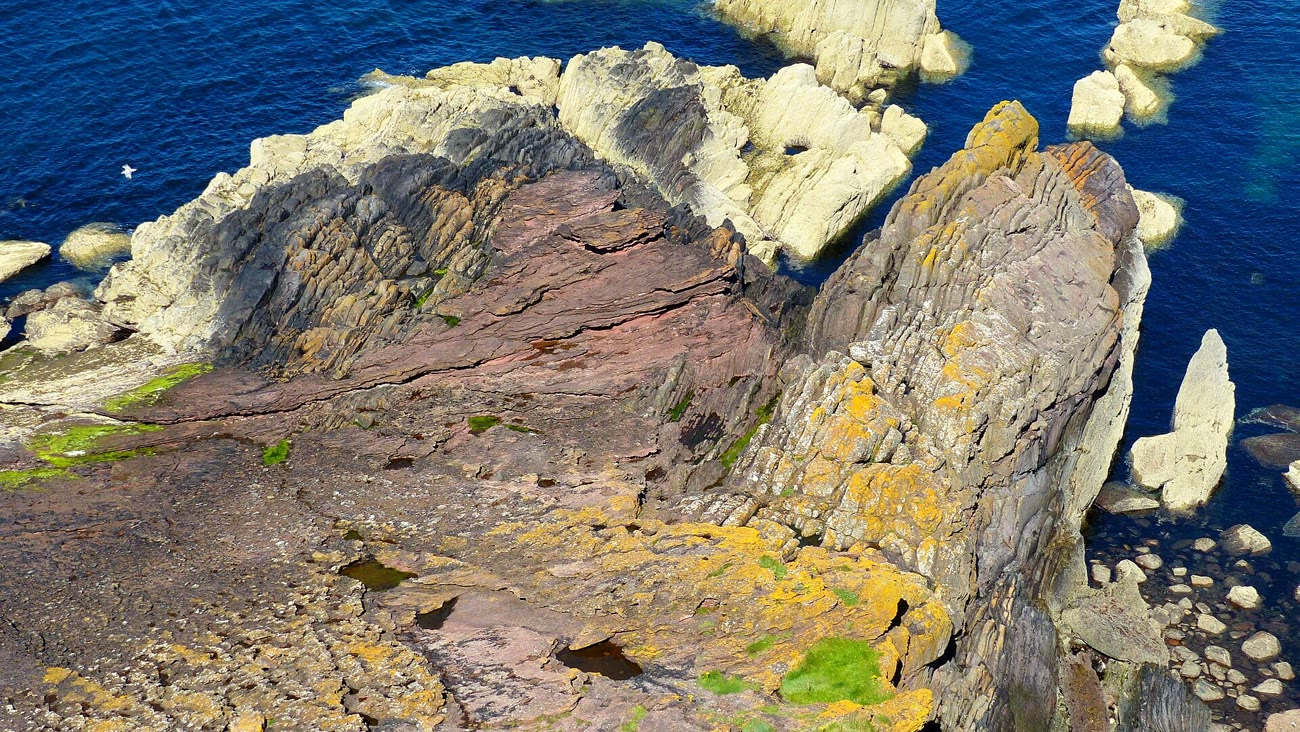
\includegraphics[width=0.7\linewidth]{images/book3/b1-siccar-point.jpg}

{\small La \omterm{def:b1:cross-sections:unconformity}{discordance} de Hutton à Siccar Point~: couches grises du Silurien
presque verticales en bas, couches rouges du Dévonien faiblement inclinées
au-dessus. Photographie PawełS, CC BY-SA 4.0 (Wikimedia Commons).}
% ledger: commons:siccar-point
\end{center}
\end{history}

\begin{inthefield}[La géologie d'un tunnel]
\begin{minipage}[t]{0.6\linewidth}\vspace{0pt}
Avant la conception d'un tunnel, les géologues de l'ingénieur construisent des
coupes le long de son tracé à partir de la \omterm{def:b1:geological-maps:geological-map}{carte géologique}, de sondages forés à
intervalles le long du parcours, et de campagnes géophysiques. Ils prévoient
chaque unité que le tunnel va recouper, les failles qu'il traversera, et les
endroits où l'eau peut entrer. Pendant le creusement, les géologues de
l'entreprise décrivent à chaque avancée la roche mise à nu au front de taille,
la comparent à la prévision et mettent la coupe à jour~; des sondages de
reconnaissance forés en avant de la machine éprouvent le terrain avant qu'elle
l'atteigne, surtout près d'une faille prévue ou dans un calcaire susceptible de
contenir des cavités. Une zone de faille de roche broyée est un danger classique,
d'autant plus quand la même roche se trouve des deux côtés et que rien au front
n'en avertit.
\end{minipage}\hfill
\begin{minipage}[t]{0.37\linewidth}\vspace{0pt}
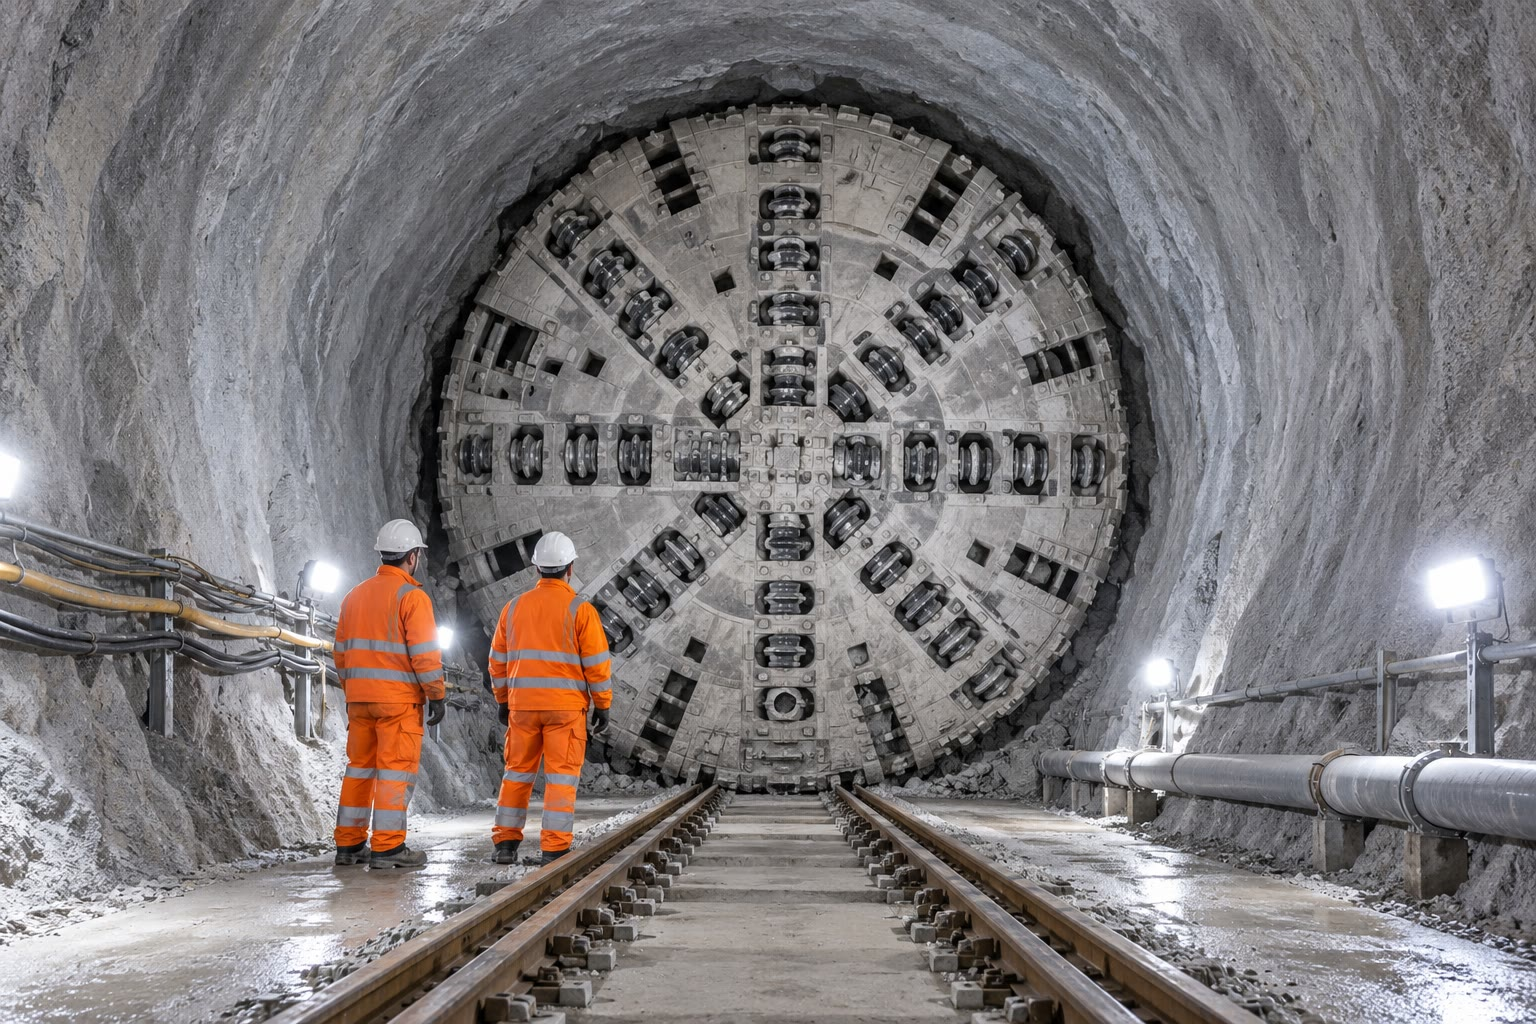
\includegraphics[width=\linewidth]{images/book3/ai/b1-tunnel-boring.jpg}
\end{minipage}
\end{inthefield}

\section{Exercices}

\begin{exercise}[$\star$]\label{exo:b1:cross-sections:1}
Une coupe est dessinée à partir d'une carte à l'échelle 1:25\,000, avec une
échelle verticale de \qty{1}{cm} pour \qty{100}{m}. Quelle est son \omterm{def:b1:cross-sections:section}{exagération
verticale}~?
\end{exercise}

\begin{exercise}[$\star$]\label{exo:b1:cross-sections:2}
Une couche plonge de \ang{40} vers \ang{090}. Quel est son \omterm{def:b1:cross-sections:apparent-dip}{pendage apparent} dans
une coupe verticale d'\omterm{def:b1:spherical-astronomy:horizontal}{azimut} \ang{060}~? D'\omterm{def:b1:spherical-astronomy:horizontal}{azimut} \ang{000}~?
\end{exercise}

\begin{exercise}[$\star$]\label{exo:b1:cross-sections:3}
Un sondage vertical traverse \qty{120}{m} de grès dont les couches plongent de
\ang{12.16}. Quelle est l'\omterm{def:b1:cross-sections:thickness}{épaisseur réelle} du grès~?
\end{exercise}

\begin{exercise}[$\star$]\label{exo:b1:cross-sections:4}
Un contact de \omterm{def:b1:geological-maps:attitude}{pendage} \ang{12} dans le plan d'une coupe est dessiné avec des
\omterm{def:b1:cross-sections:section}{exagérations verticales} de 2, 3 et 5. Sous quels angles apparaît-il~?
\end{exercise}

\begin{exercise}[$\star\star$]\label{exo:b1:cross-sections:5}
Une couche plonge de \ang{25}. Son \omterm{def:b1:geological-maps:geological-map}{affleurement} a \qty{300}{m} de large, mesurés
perpendiculairement à la direction. Calculer son \omterm{def:b1:cross-sections:thickness}{épaisseur réelle} (a) sur terrain
plat~; (b) sur un terrain incliné de \ang{10} en sens inverse du \omterm{def:b1:geological-maps:attitude}{pendage}, la
largeur étant mesurée le long du terrain~; (c) sur un terrain incliné de \ang{10}
dans le même sens que le \omterm{def:b1:geological-maps:attitude}{pendage}.
\end{exercise}

\begin{exercise}[$\star\star$]\label{exo:b1:cross-sections:6}
Une couche montre un \omterm{def:b1:cross-sections:apparent-dip}{pendage apparent} de \ang{20} vers le nord dans une coupe
nord--sud, et de \ang{30} vers l'est dans une coupe est--ouest. Trouver son \omterm{def:b1:geological-maps:attitude}{sens
du pendage} et son \omterm{def:b1:geological-maps:attitude}{pendage} réel.
\end{exercise}

\begin{exercise}[$\star\star$]\label{exo:b1:cross-sections:7}
La base du calcaire sur le flanc est plonge de \ang{12.16}. Quel est l'espacement
horizontal de ses \omterm{def:b1:cross-sections:structure-contour}{isohypses structurales} tracées tous les \qty{100}{m}~? Le
vérifier sur la \omterm{def:b1:cross-sections:structure-contour}{carte d'isohypses structurales}.
\end{exercise}

\begin{exercise}[$\star\star$]\label{exo:b1:cross-sections:8}
À partir du tableau des sondages, calculer l'altitude de la base de l'argilite en
B1 et B3. Au-dessus de B2, l'argilite a été érodée~: à partir de l'\omterm{def:b1:cross-sections:thickness}{épaisseur
verticale} du calcaire, trouver l'altitude qu'aurait sa base à cet endroit, et le
\omterm{def:b1:cross-sections:apparent-dip}{pendage apparent} de ce contact entre B1 et B2 dans la coupe C--D. Que dit la
comparaison de B1 et B3 sur le \omterm{def:b1:geological-maps:fold}{pli}~?
\end{exercise}

\begin{exercise}[$\star\star$]\label{exo:b1:cross-sections:9}
Une faille normale de \omterm{def:b1:geological-maps:attitude}{pendage} \ang{50} vers \ang{180} a un \omterm{def:b1:cross-sections:throw}{rejet vertical} de
\qty{150}{m}. Calculer son \omterm{def:b1:cross-sections:throw}{rejet horizontal}. Dans une coupe verticale d'\omterm{def:b1:spherical-astronomy:horizontal}{azimut}
\ang{150}, quels sont le \omterm{def:b1:cross-sections:apparent-dip}{pendage apparent} de la faille et la séparation des deux
traces d'une couche horizontale le long de la coupe~?
\end{exercise}

\begin{exercise}[$\star\star\star$]\label{exo:b1:cross-sections:10}
Pour une couche de \omterm{def:b1:geological-maps:attitude}{pendage} \ang{40}, dans quelles directions de coupe le \omterm{def:b1:cross-sections:apparent-dip}{pendage
apparent} vaut-il la moitié du \omterm{def:b1:geological-maps:attitude}{pendage} réel, soit \ang{20}~? Montrer que le
\omterm{def:b1:cross-sections:apparent-dip}{pendage apparent} varie peu au voisinage du \omterm{def:b1:geological-maps:attitude}{sens du pendage} et vite au voisinage
de la direction.
\end{exercise}

\begin{exercise}[$\star\star\star$]\label{exo:b1:cross-sections:11}
Un sondage traverse le calcaire du flanc est (\omterm{def:b1:cross-sections:thickness}{épaisseur réelle} \qty{176.0}{m},
\omterm{def:b1:geological-maps:attitude}{pendage} \ang{12.16} vers \ang{080.7}). Quelle longueur de carotte récupère-t-il
(a) s'il est vertical~; (b) s'il est incliné de \ang{60} sous l'horizontale vers
\ang{260.7}~; (c) incliné de \ang{60} vers \ang{080.7}~? (Indication~: la
longueur est $t/\cos\psi$, où $\psi$ est l'angle entre le sondage et la normale
à la stratification.)
\end{exercise}

\begin{exercise}[$\star\star\star$]\label{exo:b1:cross-sections:12}
À une \omterm{def:b1:cross-sections:unconformity}{discordance angulaire}, les couches inférieures plongent de \ang{70} vers
\ang{090} et les couches supérieures de \ang{20} vers \ang{270}, avec la même
direction. Faire tourner tout l'\omterm{def:b1:geological-maps:geological-map}{affleurement} autour de la direction pour ramener
les couches supérieures à l'horizontale~: quel était le \omterm{def:b1:geological-maps:attitude}{pendage} des couches
inférieures au moment du dépôt des supérieures~? Écrire dans l'ordre l'histoire
de l'\omterm{def:b1:geological-maps:geological-map}{affleurement}.
\end{exercise}

\section{Problème~: Un tunnel sous les collines de Varden}

\begin{problem}[{Problème du week-end --- quelles roches un tunnel va couper, où
il rencontrera la faille, et combien de calcaire il traversera}]
\label{pb:b1:cross-sections:1}
% numbers from figdata/bachelor-1/varden_sections.py (model region.py) and the scratch calculator
Le tunnel court plein est le long de la ligne C--D ($y = \qty{6}{km}$) à
l'altitude constante de \qty{200}{m}, de $x = \qty{1}{km}$ à $x =
\qty{9}{km}$. L'altitude du sol le long de C--D est, tous les kilomètres à
partir de $x = 0$~:
\begin{center}
\small
\begin{tabular}{lccccccccccc}
\hline
$x$ (km) & 0 & 1 & 2 & 3 & 4 & 5 & 6 & 7 & 8 & 9 & 10 \\
$z$ (m) & 509 & 556 & 467 & 370 & 435 & 534 & 501 & 455 & 406 & 339 & 405 \\
\hline
\end{tabular}
\end{center}
Utiliser le tableau des sondages du chapitre, la coupe C--D dessinée avec
$e = 3$, l'\omterm{def:b1:geological-maps:attitude}{attitude} du flanc est (\omterm{def:b1:geological-maps:attitude}{pendage} \ang{12.16} vers \ang{080.7}~; le flanc
ouest en est l'image en miroir, plongeant vers \ang{279.3}), et la faille
normale, qui plonge de \ang{60} vers \ang{120}, a un \omterm{def:b1:cross-sections:throw}{rejet vertical} de
\qty{200}{m}, et passe par le point $x = \qty{4.30}{km}$, $y = \qty{1.00}{km}$,
$z = \qty{250}{m}$.

\medskip
\noindent\textbf{Partie I --- Le profil et les unités.}
\begin{enumerate}
  \item Quelles sont la plus grande et la plus petite épaisseur de roche
        au-dessus du tunnel aux points kilométriques entre $x = 1$ et $x = 9$~?
  \item Sur la coupe imprimée, \qty{1}{km} de distance horizontale mesure
        \qty{1.4}{cm} et \qty{1}{km} d'altitude mesure \qty{4.2}{cm}. Vérifier
        que $e = 3$.
  \item D'après le log B2, trouver l'altitude de la base du grès à la crête de
        l'\omterm{def:b1:geological-maps:fold}{anticlinal}.
  \item Dans quelle unité se trouve le tunnel à $x = \qty{3.5}{km}$~?
  \item Calculer l'altitude de la base du calcaire en B1 et B3.
  \item D'après la coupe, lister dans l'ordre les unités que le tunnel traverse
        de $x = 1$ à $x = \qty{9}{km}$.
\end{enumerate}

\medskip
\noindent\textbf{Partie II --- Pendages dans la coupe.}
\begin{enumerate}[resume]
  \item Calculer le \omterm{def:b1:cross-sections:apparent-dip}{pendage apparent} du flanc est dans C--D à partir de son
        \omterm{def:b1:geological-maps:attitude}{attitude}.
  \item Le vérifier à partir des altitudes de la base du calcaire en B2 et
        B3.
  \item Sous quel angle le flanc est est-il dessiné dans la coupe à $e = 3$~?
  \item Calculer le \omterm{def:b1:cross-sections:apparent-dip}{pendage apparent} de la faille dans C--D.
  \item Pourquoi le \omterm{def:b1:cross-sections:apparent-dip}{pendage apparent} des flancs dans C--D est-il si proche de
        leur \omterm{def:b1:geological-maps:attitude}{pendage} réel, et celui de la faille moins~?
\end{enumerate}

\medskip
\noindent\textbf{Partie III --- La faille.}
\begin{enumerate}[resume]
  \item Montrer que, dans le plan $y = \qty{6}{km}$, la faille se trouve en
        \[ x = 4300 + \frac{2500 - (z - 250)\tan\ang{30}}{\sin\ang{120}}
           \quad\text{(mètres)}. \]
  \item Où le tunnel rencontre-t-il la faille~?
  \item Calculer le \omterm{def:b1:cross-sections:throw}{rejet horizontal} de la faille, et la séparation des deux
        points où un contact la rencontre le long de C--D.
  \item Quel bloc est affaissé, et quelle unité se trouve au niveau du tunnel de
        chaque côté de la faille~?
  \item Pourquoi la faille est-elle un danger que l'équipe de creusement ne
        pourrait pas deviner d'après la roche au front~? Comment les ingénieurs
        s'en prémunissent-ils~?
\end{enumerate}

\medskip
\noindent\textbf{Partie IV --- Le calcaire.}
\begin{enumerate}[resume]
  \item Quelle est l'\omterm{def:b1:cross-sections:thickness}{épaisseur verticale} du calcaire en B1~?
  \item Quelle est son \omterm{def:b1:cross-sections:thickness}{épaisseur réelle}~?
  \item Montrer que, à l'ouest de la faille sur C--D, la base du grès se trouve
        à
        \[ z_b = 160.16 - |x - 3500|\tan\ang{12.0} \quad\text{(mètres)}. \]
  \item Le tunnel est dans le calcaire lorsque sa base est au-dessous de
        \qty{200}{m} et son toit au-dessus. Montrer que cela se produit pour
        $377.1 < |x - 3500|
        < 1224.0$.
  \item Donner les quatre points où le tunnel entre dans le calcaire et en sort.
  \item Montrer que la longueur creusée sur chaque flanc est $h/\tan\beta$, où
        $h$ est l'\omterm{def:b1:cross-sections:thickness}{épaisseur verticale} et $\beta$ le \omterm{def:b1:cross-sections:apparent-dip}{pendage apparent}, et la
        calculer.
  \item Quelle longueur totale de calcaire le tunnel traverse-t-il~?
\end{enumerate}
\end{problem}
